%%%%%%%%%%%%%%%%%%%%%%%%%%%%%%%%%%%%%%%%%
% Beamer Presentation
% LaTeX Template
% Version 1.0 (10/11/12)
%
% This template has been downloaded from:
% http://www.LaTeXTemplates.com
%
% License:
% CC BY-NC-SA 3.0 (http://creativecommons.org/licenses/by-nc-sa/3.0/)
%
%%%%%%%%%%%%%%%%%%%%%%%%%%%%%%%%%%%%%%%%%

 
%----------------------------------------------------------------------------------------
%	PACKAGES AND THEMES
%----------------------------------------------------------------------------------------

\documentclass{beamer}
\usepackage[utf8]{inputenc}
\usepackage{amsmath}
\usepackage{graphicx}
\usepackage{hyperref}
\usepackage{float}
\usepackage{wrapfig}
\usepackage{comment} % enables the use of multi-line comments (\ifx \fi) 
\usepackage{lipsum} %This package just generates Lorem Ipsum filler text.
\usepackage[french]{babel}

\mode<presentation> {

% The Beamer class comes with a number of default slide themes
% which change the colors and layouts of slides. Below this is a list
% of all the themes, uncomment each in turn to see what they look like.

%\usetheme{default}
%\usetheme{AnnArbor}
%\usetheme{Antibes}
%\usetheme{Bergen}
%\usetheme{Berkeley}
%\usetheme{Berlin}
%\usetheme{Boadilla}
%\usetheme{CambridgeUS}
%\usetheme{Copenhagen}
%\usetheme{Darmstadt}
%\usetheme{Dresden}
%\usetheme{Frankfurt}
%\usetheme{Goettingen}
%\usetheme{Hannover}
%\usetheme{Ilmenau}
%\usetheme{JuanLesPins}
%\usetheme{Luebeck}
%\usetheme{Madrid}
%\usetheme{Malmoe}
%\usetheme{Marburg}
%\usetheme{Montpellier}
%\usetheme{PaloAlto}
%\usetheme{Pittsburgh}
%\usetheme{Rochester}
\usetheme{Singapore}
%\usetheme{Szeged}
%\usetheme{Warsaw}

% As well as themes, the Beamer class has a number of color themes
% for any slide theme. Uncomment each of these in turn to see how it
% changes the colors of your current slide theme.

%\usecolortheme{albatross}
%\usecolortheme{beaver}
%\usecolortheme{beetle}
%\usecolortheme{crane}
%\usecolortheme{dolphin}
%\usecolortheme{dove}
%\usecolortheme{fly}
%\usecolortheme{lily}
%\usecolortheme{orchid}
%\usecolortheme{rose}
%\usecolortheme{seagull}
%\usecolortheme{seahorse}
%\usecolortheme{whale}
%\usecolortheme{wolverine}

%\setbeamertemplate{footline} % To remove the footer line in all slides uncomment this line
%\setbeamertemplate{footline}[page number] % To replace the footer line in all slides with a simple slide count uncomment this line

%\setbeamertemplate{navigation symbols}{} % To remove the navigation symbols from the bottom of all slides uncomment this line
}

\usepackage{graphicx} % Allows including images
\usepackage{booktabs} % Allows the use of \toprule, \midrule and \bottomrule in tables

%----------------------------------------------------------------------------------------
%	TITLE PAGE
%----------------------------------------------------------------------------------------

\title{Projet MAP512 - Problème de flots à coût minimum avec contraintes de gradient : optimisation de la production d'une vallée fluviale au cours du temps} % The short title appears at the bottom of every slide, the full title is only on the title page

\author{Augustin Thomas et Pimprenelle Parmentier} % Your name



\date{\today} % Date, can be changed to a custom date



\begin{document}

\begin{frame}
\titlepage % Print the title page as the first slide
\insertframenumber\end{frame}

\begin{frame}
\frametitle{Plan} % Table of contents slide, comment this block out to remove it
\tableofcontents % Throughout your presentation, if you choose to use \section{} and \subsection{} commands, these will automatically be printed on this slide as an overview of your presentation
\insertframenumber\end{frame}

%----------------------------------------------------------------------------------------
%	PRESENTATION SLIDES
%----------------------------------------------------------------------------------------

%------------------------------------------------

\section{Introduction} % Sections can be created in order to organize your presentation into discrete blocks, all sections and subsections are automatically printed in the table of contents as an overview of the talk

\begin{frame}{Introduction}

\begin{figure}[H]
    \begin{minipage}[c]{.46\linewidth}
        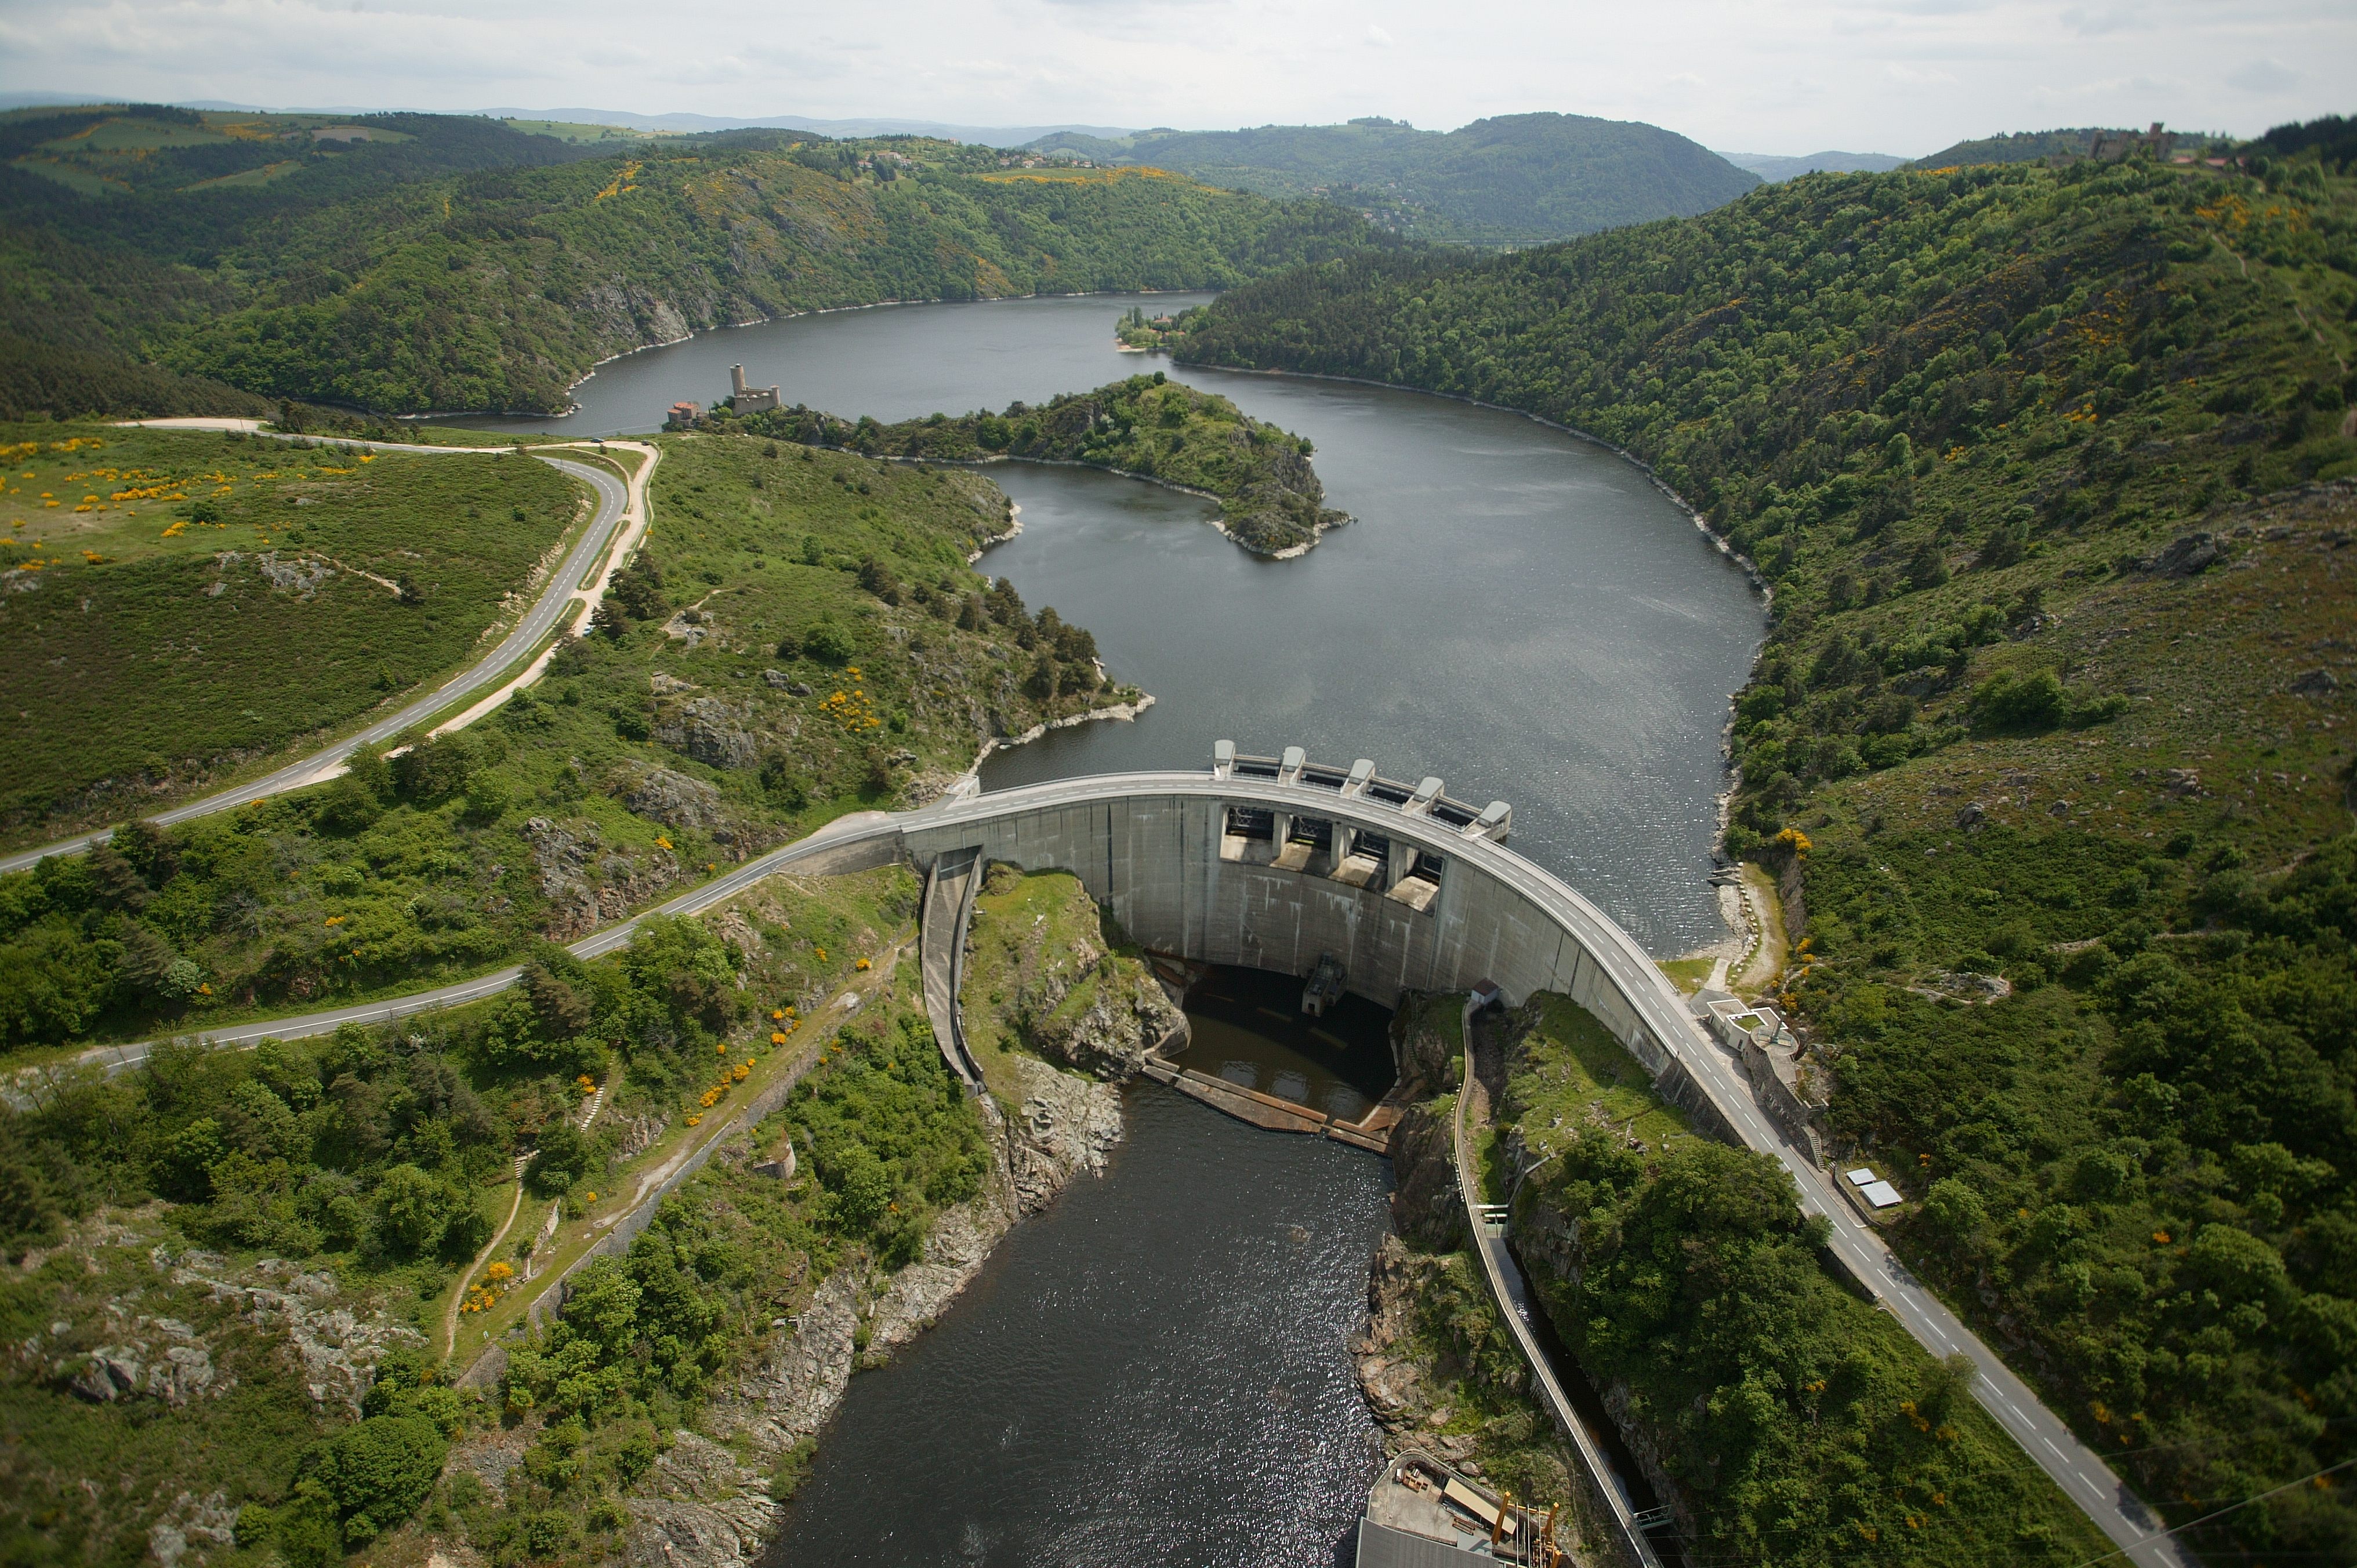
\includegraphics[width=5cm]{barragephoto.jpg}
        \caption{Le barrage de Grangent, Loire}
        \label{fig:simplexe}
    \end{minipage} \hfill
    \begin{minipage}[c]{.46\linewidth}
        \includegraphics[width=5cm]{carto_hydroelec_Lot.png}
        \caption{exemple de bassin hydrographique et ses barrages}
        \label{carto}
    \end{minipage}
\end{figure}

\insertframenumber
\end{frame}
%------------------------------------------------
\section{Présentation du problème et état de l'art}
\subsection{Modélisation}
\begin{frame}{Présentation du problème et état de l'art : Modélisation}
\begin{figure}[h]
    \centering
    \includegraphics[width = 9cm]{barrageexemple.JPG}
    \caption{Modélisation d'un barrage dans une vallée}
    \label{fig:exemple}
\end{figure}
Notre jeu de contraintes : 
\begin{itemize}
    \item contraintes de Kirchhoff
    \item contraintes Up\&Min
    \item \textbf{contraintes de gradient}
\end{itemize}

\insertframenumber\end{frame}

\subsection{Problème linéaire}
\begin{frame}{Un problème linéaire}

$$
    \displaystyle \min_{ \left\{
    \begin{array}{ll}
         A ^t X = ^t B \\
          Min\leq X\leq Up\\
          ^t G_{min} \leq ^tD X \leq ^t G_{max} 
    \end{array}
    \right.
    }
    {^t C X}
$$
\begin{itemize}
    \item $X$ : flot sur les arcs (taille n)
    \item $C$ : cout sur chaque arc (taille n)
    \item $A$ : contraintes de Kirchhoff (taille k = nombre de noeuds - 1)
    \item $Min$ et $Up$ : vecteurs contraintes Up\&Min
    \item $G_{min}$ et $G_{max}$ : vecteurs contraintes de gradient; $^tDX$ : calcul du gradient
\end{itemize}
\insertframenumber\end{frame}


\begin{frame}{Méthode du simplexe}

\begin{figure}[H]
    \begin{minipage}[c]{.66\linewidth}
        \includegraphics[width=10cm]{simplexe.jpg}
        \caption{Le polyèdre associé à l'algorithme du simplexe}
        \label{fig:simplexe}
    \end{minipage} \hfill
    \begin{minipage}[c]{.26\linewidth}
        La solution du problème correspond à un ensemble de taille $n$ de contraintes saturées (un sommet du polyèdre).
    \end{minipage}
\end{figure}
\insertframenumber\end{frame}


\begin{frame}{Résolution du problème de flot à coût minimal sans contraintes de gradient : un exemple}
    \begin{figure}[h]
    \centering
        \includegraphics[width=7cm]{exemplesanscontchiffre.JPG}
        \caption{Un exemple de graphe avec les coûts (en gros) et les contraintes \textit{Up\&Min}}
        \label{fig:exsansgrad}
    \end{figure}
\insertframenumber\end{frame}



\begin{frame}{Résolution du problème de flot à coût minimal sans contraintes de gradient : un exemple}
    \begin{figure}
        \centering
        \includegraphics[width = 7cm]{solsanscont.JPG}
        \caption{Entouré : les flots solution du problème de flot à coût minimal. En rouge : les arêtes où les contraintes sont saturées.}
        \label{fig:resosansgrad}
    \end{figure}    
    Résolution en $O(n)$
\insertframenumber\end{frame}

\subsection{Adaptation aux contraintes de gradient}

\begin{frame}{Adaptation aux contraintes de gradient}
    \begin{figure}[H]
        \centering
        \includegraphics[width=10cm]{ajoutgrad.JPG}
        \caption{Ajout des contraintes de gradient.}
        \label{fig:ajoutcontgrad}
    \end{figure}
\insertframenumber
\end{frame}

\begin{frame}{Adaptation aux contraintes de gradient}
    \begin{figure}[H]
        \centering
        \includegraphics[width=6cm]{cyclessanssol.JPG}
        \caption{On va ajuster les solutions de la figure \ref{fig:ajoutcontgrad} à l'aide de deux cycles $\lambda_1$ et $\lambda_2$. }
        \label{fig:cycles}


    \end{figure}
    Système associé : 
    $$
    \left(
    \begin{matrix}
    (2+\lambda_1 - \lambda_2 ) & - & (1-\lambda_1) & = & 2\\
    (7+\lambda_2) & - & (2-\lambda_2 + \lambda_1) & = & 2
    \end{matrix}\right)
    \Rightarrow
    \left(
    \begin{matrix}
    \lambda_1 &=& -\frac{1}{3}\\
    \lambda_2 & = & -\frac{5}{3}
    \end{matrix}\right)
    $$
\insertframenumber\end{frame}
\begin{frame}{Adaptation aux contraintes de gradient}
    \begin{figure}[H]
        \centering
        \includegraphics[width=10cm]{solfinale.JPG}
        \caption{Le flot final.}
        \label{fig:solfinale}
    \end{figure}
\insertframenumber\end{frame}

\section{Choix des cycles}
\subsection{Tentative de simplification pour une vallée fluviale linéaire}
\begin{frame}{Tentative de simplification pour une vallée fluviale linéaire}

\begin{figure}[H]
    \centering
    \includegraphics[width = 8cm]{valleelineaire.jpg}
    \caption{Cas d'une vallée fluviale linéaire}
    \label{fig:valleefluvialelineaire}
\end{figure}

\insertframenumber\end{frame}

\begin{frame}{Méthode des cycles imbriqués}

\begin{figure}[H]
    \centering
    \includegraphics[width = 10cm]{Graphe_ligne_cycles.jpg}
    \caption{Une "ligne" où on a représenté une base de cycles imbriqués. Son système associé est: 
    \centering
    $$ \begin{matrix}
            2 \lambda_1  & + \lambda_2  &+ \lambda_3 & + \lambda_4 & = & 0 \\
            - \lambda_1 & + \lambda_2 & & & = & 0 \\
            & - \lambda_2 & + \lambda_3 & & = & 0 \\
            & & - \lambda_3 & + \lambda_4 & = & 0
        \end{matrix} $$
    }
    \label{fig:Uneligne}
\end{figure}
    
\insertframenumber\end{frame}

\subsection{Contre exemple}

\begin{frame}{Contre exemple}
    

\begin{figure}[H]
    \centering
    \includegraphics[width = 7cm]{contre_exemple.jpg}
    \caption{Contre exemple. Dans le cas général, on peut obtenir un système de forme quelconque}
    \label{fig:Contreexemple}
\end{figure}

\insertframenumber\end{frame}

\section{Résolution par mise à jour incrémentale}
\subsection{Cadre d'application de la mise à jour incrémentale avec la méthode de Bartels-Golub}
\begin{frame}{Méthode de Bartels-Golub}

On dispose à l'étape i d'une matrice B, de taille $n_B$, et des matrices suivantes:
$$M_{r}M_{r-1}\dots M_1 B = PUQ$$

\begin{itemize}
    \item $U$ est une matrice triangulaire supérieure
    \item $M_{r},M_{r-1},\dots M_1$ sont des matrices $I + \alpha_r E_{i_r,j_r}$, correspondant à l'opération $L_{i_r} \leftarrow L_{i_r} + \alpha_r \times L_{j_r}$
    \item $P$ est une matrice de permutation sur les lignes
    \item $Q$ est une matrice de permutation sur les colonnes.
\end{itemize}

Si on note $S$ une matrice dont une colonne diffère de B, alors on obtient à l'étape i+1 :
$$M_{r}M_{r-1}\dots M_1 S = P\bar{U}Q$$
\insertframenumber\end{frame}


\begin{frame}{Méthode de Bartels-Golub}
\begin{figure}[H]
\centering
    \begin{minipage}[c]{.46\linewidth}
    \includegraphics[width=4cm]{matricepic.JPG}
    \caption{La matrice $\bar{U}$}
    \label{fig:pic}
    \end{minipage} \hfill
    \begin{minipage}[c]{.46\linewidth}
    \includegraphics[width = 4cm]{bartelgolub.JPG}
    \caption{$\bar{U}$ après permutation}
    \label{fig:Bartelsgolub}
    \end{minipage} \hfill
\end{figure}

Après permutation dans la matrice $\bar{U}$, on supprime la sous-diagonale en $n^2$ opérations. 

\insertframenumber\end{frame}

\begin{frame}{Cas de mise à jour : une méthode pas tout à fait adaptée}
    Ici, quatre cas de mise à jour sont possibles : \begin{enumerate}
    \item on relâche une contrainte de gradient pour saturer une contrainte "Up\&Min" ($Cg \rightarrow UM$ : on retire donc une ligne et une colonne de la matrice.) \pause \textbf{$\rightarrow$ BG non exploitable}\pause
    \item on relâche une contrainte "Up\&Min" pour saturer une contrainte de gradient ($Um \rightarrow Gg$ : on ajoute une ligne et une colonne à la matrice.)\pause \textbf{$\rightarrow$ BG exploitable} \pause
    \item on relâche une contrainte de gradient pour en saturer une autre ( $Gd \rightarrow Gd$: : une ligne de la matrice est modifiée.) \pause \textbf{$\rightarrow$ BG non exploitable}\pause
    \item on relâche une contrainte "Up\&Min" et on en sature une autre ($Um \rightarrow Um$ : on change quelques colonnes de B). \pause \textbf{$\rightarrow$ BG exploitable sous réserve d'avoir un arbre couvrant initial compatible}
\end{enumerate}
\insertframenumber
\end{frame}

\begin{frame}{Choix des cycles}
    \begin{figure}[H]
        \centering
        \includegraphics[width=8cm]{coloriage.JPG}
        \caption{Un exemple de "coloriage" et de ses cycles associés.}
        \label{fig:coloriage}
    \end{figure}
\insertframenumber
\end{frame}

\begin{frame}{Une structure particulière à exploiter}
    \begin{figure}[H]
    \centering
    \includegraphics[width=10cm]{arbrecontraintes.JPG}
    \caption{Un exemple de structure}
    \label{fig:pseudoarbre}
\end{figure}
\insertframenumber\end{frame}
\begin{frame}{L'algorithme}
    \begin{enumerate}
        \item Données: contraintes de Kirchhoff saturées, contraintes Up\&Min, contraintes de gradient,  coûts, flots entrants.
        \item Initialisation: on représente le graphe de façon planaire. 
        \item Boucle $i$: Déterminer les contraintes à saturer.
        \item Arbre couvrant de contraintes non saturées Up\&Min
        \item On calcule les flots sur le graphe correspondant à cet arbre.
        \item On détermine les cycles et la matrice $B_i$ des contraintes à résoudre.
        \item Bartel-Golub en fonction des matrices déjà parcourues pour calculer $B_i^{-1}$
        \item Revenir en début de boucle.
    \end{enumerate}
\insertframenumber\end{frame}

\section{Conclusion}
\begin{frame}{Conclusion}
    \begin{itemize}
        \item Résultats: 
        \begin{itemize}
            \item Impossibilité de choisir une base de cycles adaptée dans le cas général
            \item Amélioration relative de la complexité par mise à jour incrémentale $\rightarrow$ dépend du chemin suivi dans le pseudo-arbre
        \end{itemize}
        \item Pistes d'amélioration :
            \begin{itemize}
                \item choix des contraintes : créer une heuristique à ajouter aux coûts réduits pour le choix du prochain sommet à visiter dans l'algorithme du simplexe ?
                \item coloriage de graphe : théoriquement intéressant, mais pas facile à coder en pratique.
                \item plus généralement : coder et tester l'algorithme
            \end{itemize}
    \end{itemize}
    
\end{frame}

\begin{frame}{Bibliographie}
\nocite{*}
\bibliographystyle{alpha}
\bibliography{main}

\insertframenumber\end{frame}

\end{document}